\newpage 

\section{Results}

\subsection{Classification}

Our network converges after training for 20 epochs. To evaluate performance, we observe that the test accuracy on recognizable samples is 0.88, which is very high for a small proof-of-concept network. A traditional CNN of similar architecture was trained alongside the BCNN to compare performance between both models. Test accuracies were comparable with the CNN outperforming the BCNN by 2 percentage points. This difference is negligible in practice. More important is the fact that the former is a complete black box for which there is no method to derive prediction confidence from in production. Thus, even with a slightly lower test performance, the BCNN can be considered more interpretable, and therefore, more useful in practice.


\subsection{Thresholded Prediction}

To demonstrate the confidence of a BCNN, we only perform prediction on examples that we are confident about. Thus, we set a threshold of 0.2 representing the minimum belief required by the network to make a prediction about a clothing item. Any confidence of an item's class below this value is deemed unrecognizable and is not given a label during testing. Figure \ref{fig:familiar_example} shows an easily identifiable pair of pants while Figure \ref{fig:familiar_example_confidence} displays the final dense layer's distributions of confidence for each class. Notice that the mean probability of the Trousers class is both above 0.2 and is the maximally likely estimate for the given data. Therefore the network correctly predicts that the image belongs to the Trousers class. Similarly, on unfamiliar data (Figure \ref{fig:unfamiliar_example}), the BCNN fails to provide a prediction for the out-of-dataset number as no class reaches the median confidence threshold required to output a label (Figure \ref{fig:unfamiliar_example_confidence}).


\begin{figure}[!htb]
\centering
\begin{subfigure}{.5\textwidth}
  \centering
  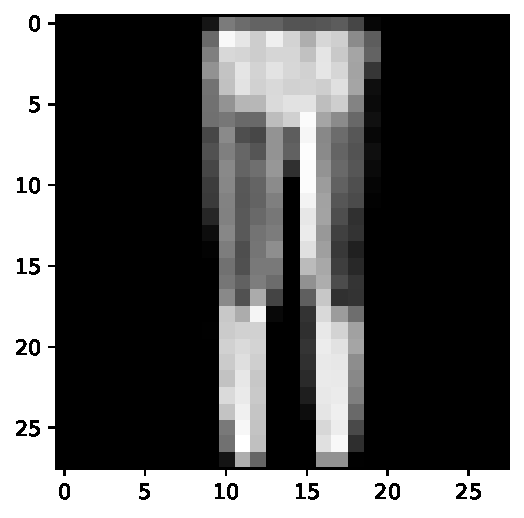
\includegraphics[scale=0.5]{Figures/familiar_example.pdf}
  \caption{Familiar Example}
  \label{fig:familiar_example}
\end{subfigure}%
\begin{subfigure}{.5\textwidth}
    \centering
    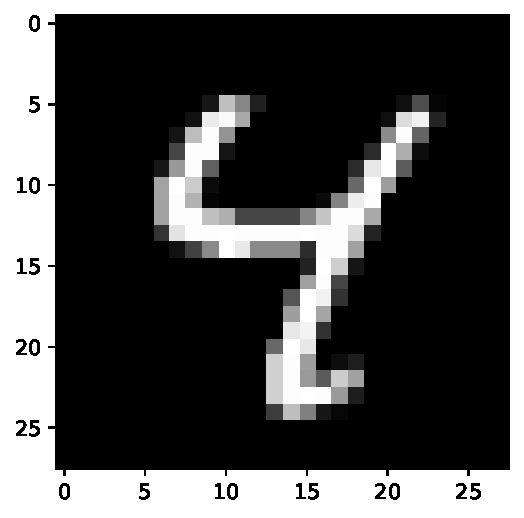
\includegraphics[scale=0.5]{Figures/MNIST_digit.pdf}
    \caption{Unfamiliar Example}
    \label{fig:unfamiliar_example}
\end{subfigure}
\caption{Examples of Familiar and Unfamiliar Data}
\label{fig:examples}
\end{figure}

\begin{figure}[!htb]
  \centering
  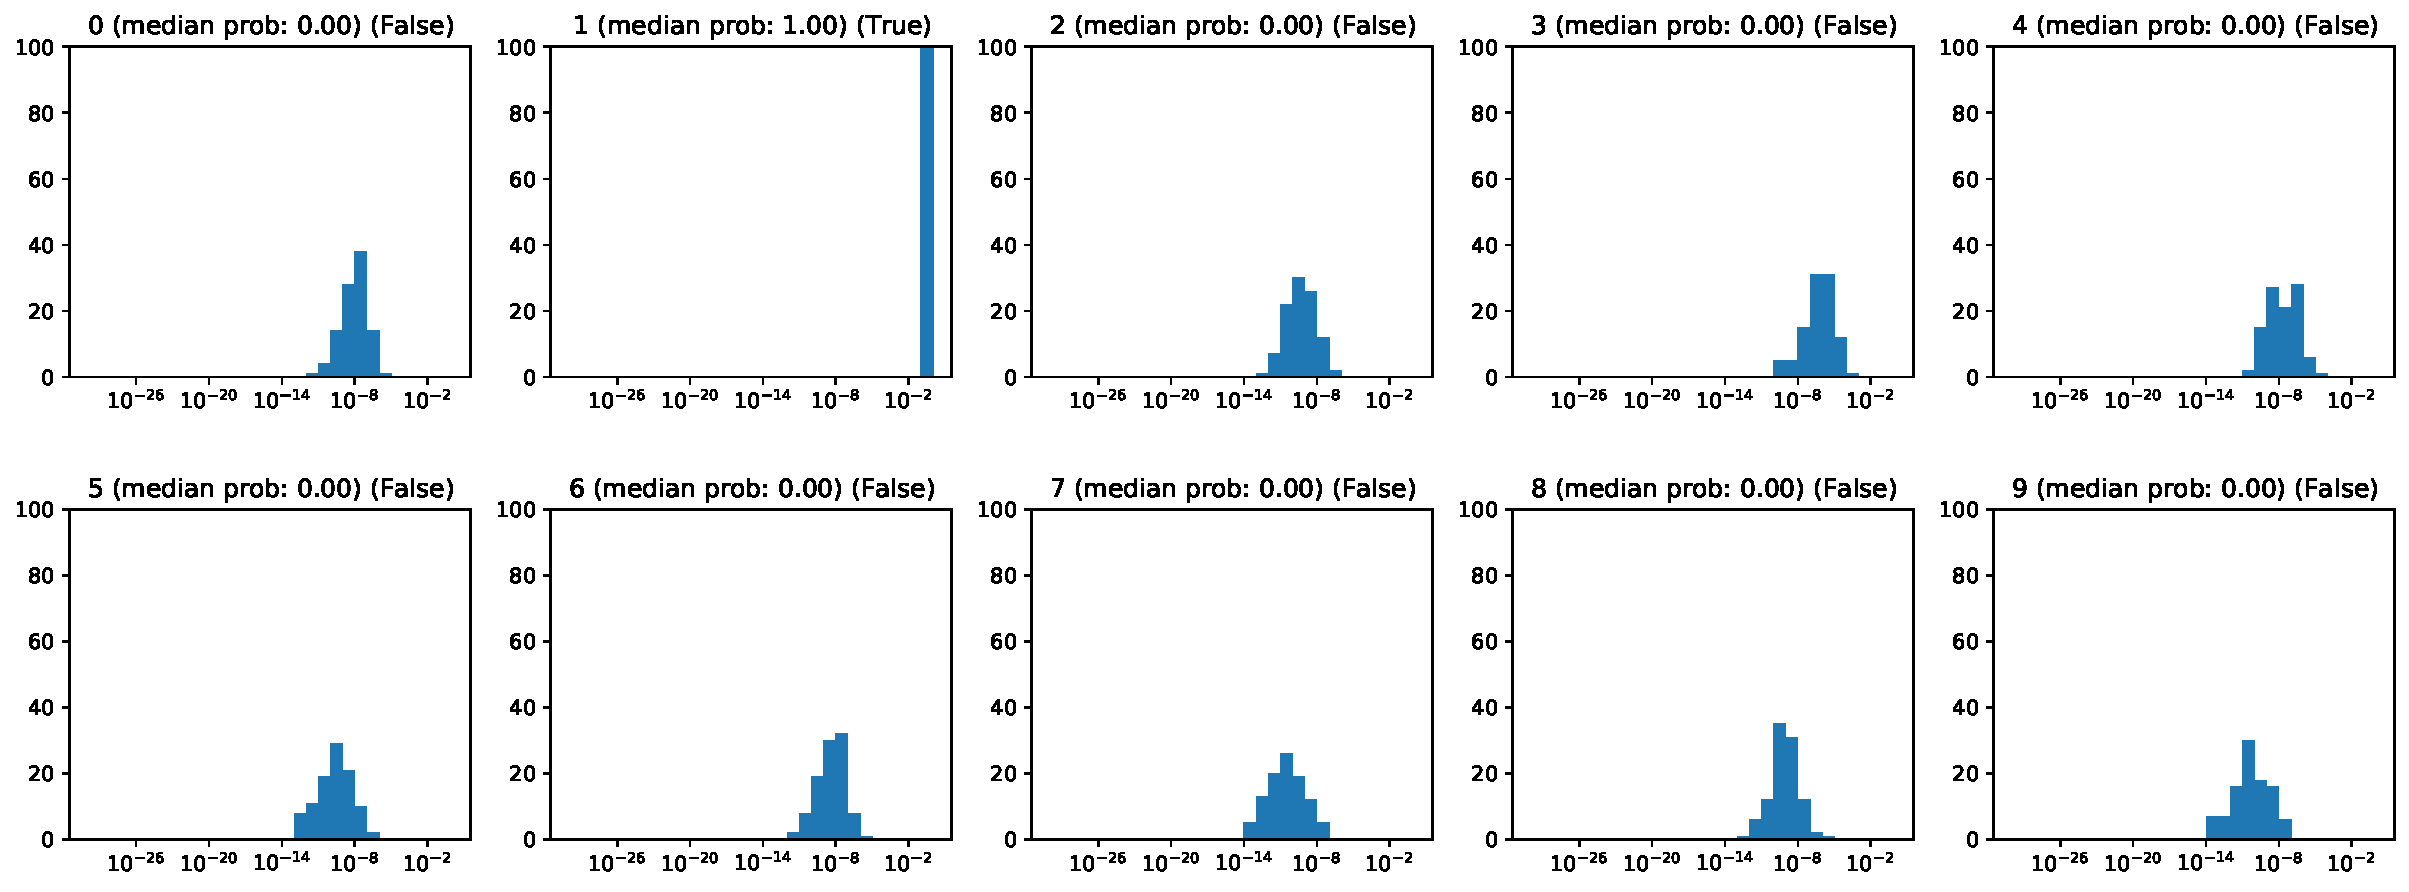
\includegraphics[width=\columnwidth]{Figures/familiar_example_confidence.pdf}
  \caption{Familiar Example Confidence Estimates}
  \label{fig:familiar_example_confidence}
\end{figure}

\begin{figure}[!htb]
  \centering
  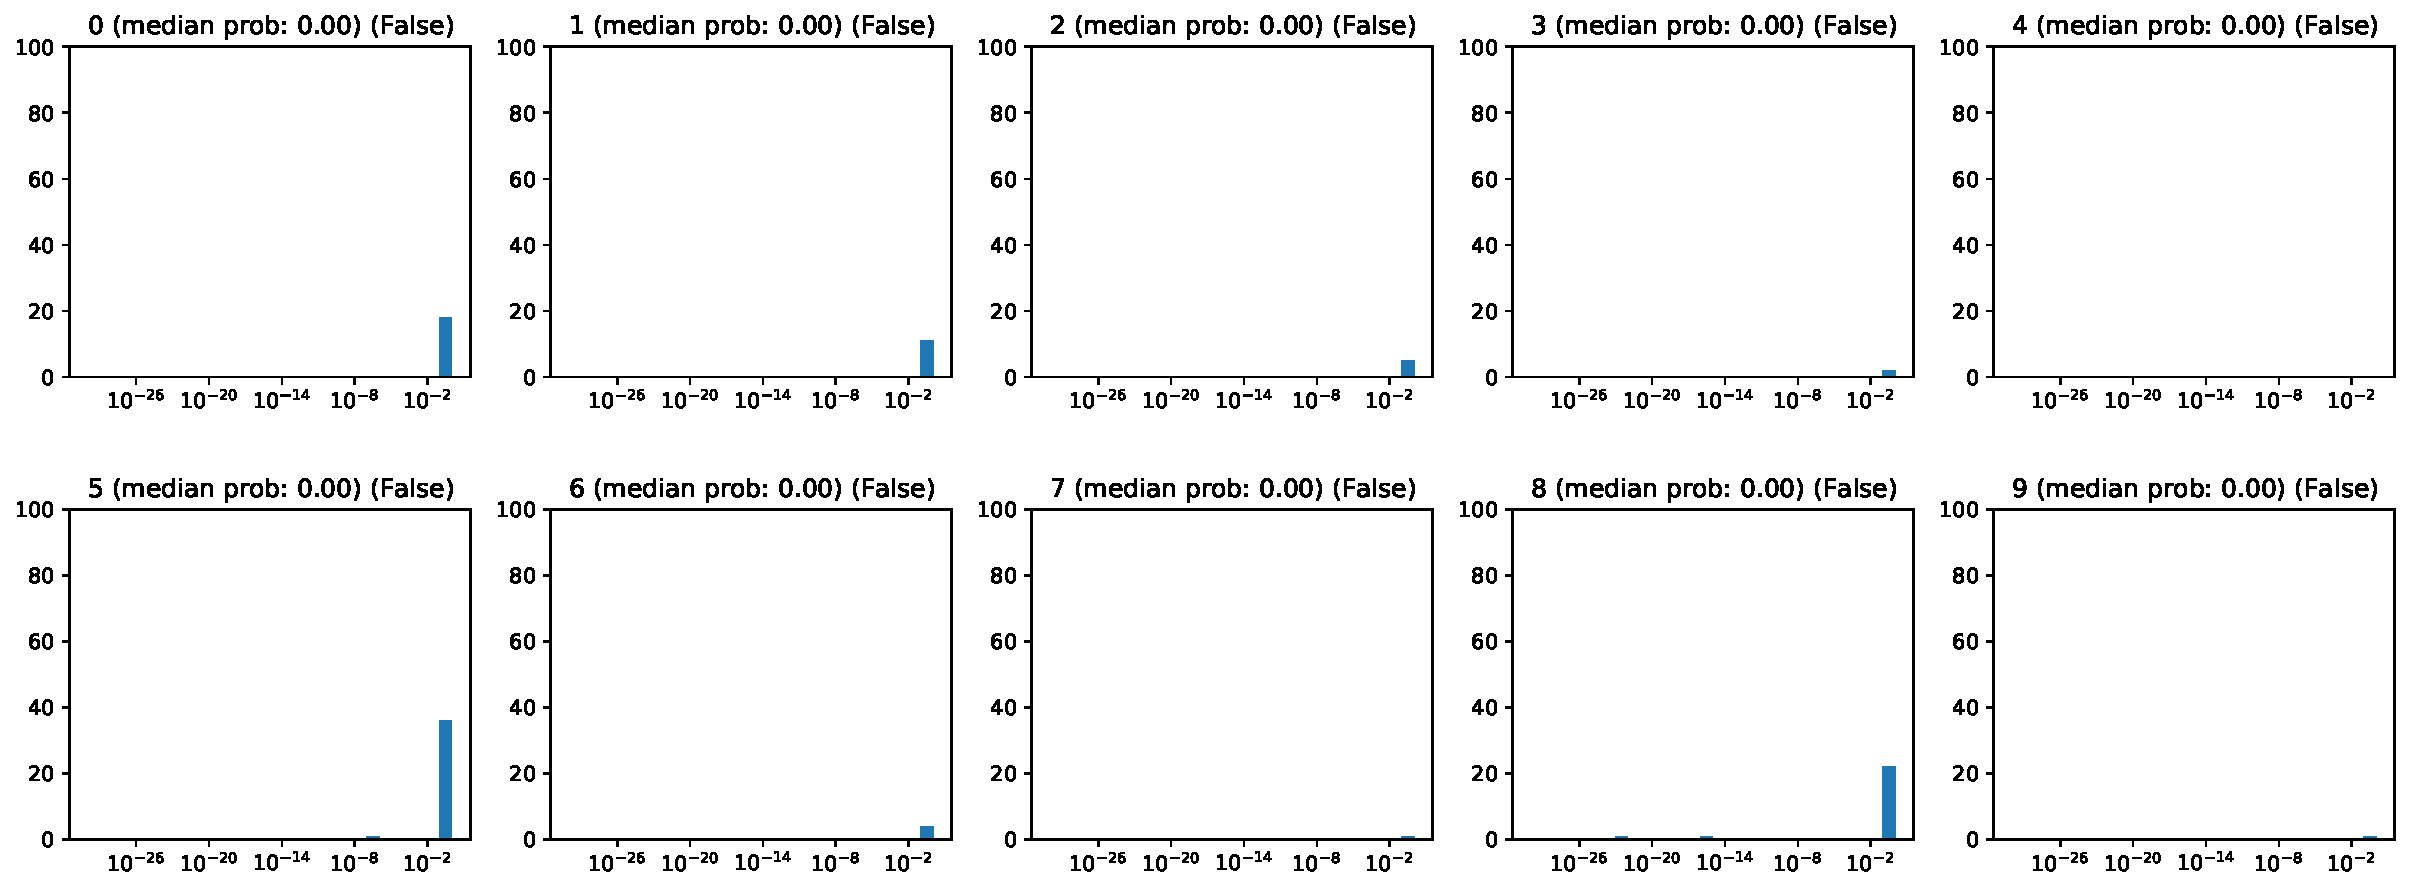
\includegraphics[width=\columnwidth]{Figures/mnist_confidence.pdf}
  \caption{Unfamiliar Example Confidence Estimates}
  \label{fig:unfamiliar_example_confidence}
\end{figure}

